\chapter{The Euler Tour Technique}

A tree is a two-dimensional object: it branches, it has depth, it has subtrees
nested inside subtrees. An array is one-dimensional: a flat row of cells you can
index, prefix-sum, and slice. The Euler tour technique is the bridge between the
two. It takes a rooted tree, walks around it in a single fixed order, and writes
down what it sees, producing an array in which \emph{every subtree occupies one
contiguous block}. Once a subtree is a contiguous block, ``update everything below
$v$'' and ``sum everything below $v$'' become range operations, and you can throw
the full arsenal of array data structures -- prefix sums, Fenwick trees (BITs),
segment trees, sparse tables -- at problems that were phrased on a tree.

The same walk, recorded slightly differently, gives the \emph{Euler tour trees} of
Henzinger and King: a representation of a forest as a balanced binary search tree
keyed on the tour, in which linking two trees, cutting an edge, and testing whether
two vertices are connected each cost $\Oh(\log n)$. That makes the Euler tour the
data-structural backbone of dynamic connectivity in forests.

This chapter builds both layers from the ground up. We flatten a small tree by
hand, watch the in/out timestamps appear, prove the contiguous-subtree theorem,
combine the flattening with a Fenwick tree to answer subtree and (with a twist)
path queries, and finally develop Euler tour trees as a dynamic forest structure.

\chapterline

\section{Flattening a tree}
\label{ch21:flatten}

Fix a rooted tree $T=(V,E)$ with $n=\abs{V}$ vertices, root $r$, and for each vertex
a fixed order on its children (any order will do; we just commit to one). Run a depth
first search from $r$. Two natural things happen as the DFS proceeds: we \emph{enter}
a vertex when we first reach it, and we \emph{leave} it when we have finished all of
its descendants and are about to return to its parent.

\begin{intuitionbox}
Imagine walking around the outside of the tree with your left hand always touching an
edge, the way you would trace a maze wall. You enter a vertex from above, dive into
its leftmost subtree, come back, dive into the next subtree, and so on, and only when
every subtree is exhausted do you climb back to the parent. The list of ``first time I
touched each vertex,'' read in the order you touched them, is the Euler tour. The
crucial fact is purely topological: while you are anywhere inside $v$'s subtree, you
have entered $v$ but not yet left it. Entry and exit \emph{bracket} the subtree like
matched parentheses.
\end{intuitionbox}

Here is the running example we will use throughout. The root is $1$; children are
listed left to right in increasing order.

\begin{center}
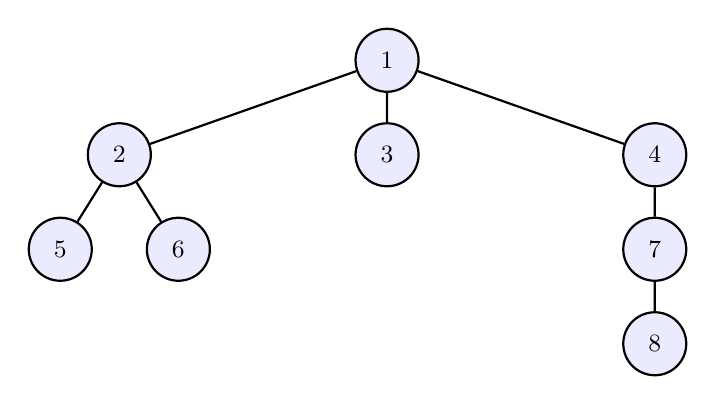
\begin{tikzpicture}[every node/.style={circle,draw,fill=blue!8,minimum size=8mm,inner sep=0pt,font=\small},level distance=12mm,thick,
  level 1/.style={sibling distance=34mm},
  level 2/.style={sibling distance=15mm}]
  \node (n1) {$1$}
    child {node (n2) {$2$}
      child {node (n5) {$5$}}
      child {node (n6) {$6$}}
    }
    child {node (n3) {$3$}}
    child {node (n4) {$4$}
      child {node (n7) {$7$}
        child {node (n8) {$8$}}
      }
    };
\end{tikzpicture}
\end{center}

There are two common ways to record the walk, and they serve different purposes. We
treat each in turn.

\subsection{The in/out timestamp encoding}

Maintain a global counter \texttt{timer}, starting at $1$. When DFS first enters a
vertex $v$, assign $\texttt{tin}[v]\leftarrow\texttt{timer}$ and increment the timer.
When DFS finishes $v$ (after all children are done), assign $\texttt{tout}[v]
\leftarrow\texttt{timer}$ and increment again. Every vertex thus receives two distinct
stamps, and the counter runs from $1$ to $2n$.

\begin{algorithm}[H]
\caption{In/out timestamps via DFS}
\label{ch21:alg-tinout}
\DontPrintSemicolon
\SetKwProg{Fn}{function}{:}{}
\KwIn{rooted tree $T$, root $r$}
\KwOut{arrays $\texttt{tin},\texttt{tout}$}
$\texttt{timer}\leftarrow 1$\;
\Fn{\textsc{DFS}$(v,\,\text{parent }p)$}{
  $\texttt{tin}[v]\leftarrow \texttt{timer}$;\quad $\texttt{timer}\leftarrow \texttt{timer}+1$\;
  \ForEach{child $c$ of $v$ with $c\neq p$}{
    \textsc{DFS}$(c,v)$\;
  }
  $\texttt{tout}[v]\leftarrow \texttt{timer}$;\quad $\texttt{timer}\leftarrow \texttt{timer}+1$\;
}
\textsc{DFS}$(r,\,\textsc{nil})$\;
\end{algorithm}

Run it by hand on the example. The DFS visits $1,2,5,6,3,4,7,8$ on the way down and
unwinds in the mirror order. The counter steps once on every enter and once on every
leave, so the sequence of events in time order is
\[
1_{\text{in}},2_{\text{in}},5_{\text{in}},5_{\text{out}},6_{\text{in}},6_{\text{out}},
2_{\text{out}},3_{\text{in}},3_{\text{out}},4_{\text{in}},7_{\text{in}},8_{\text{in}},
8_{\text{out}},7_{\text{out}},4_{\text{out}},1_{\text{out}},
\]
which assigns the stamps $1,2,\dots,16$ in that order:

\begin{center}
\begin{tabular}{c|cccccccc}
\toprule
vertex $v$ & $1$ & $2$ & $3$ & $4$ & $5$ & $6$ & $7$ & $8$\\
\midrule
$\texttt{tin}[v]$  & $1$  & $2$ & $8$  & $10$ & $3$ & $5$ & $11$ & $12$\\
$\texttt{tout}[v]$ & $16$ & $7$ & $9$  & $15$ & $4$ & $6$ & $14$ & $13$\\
\bottomrule
\end{tabular}
\end{center}

Every pair $(\texttt{tin}[v],\texttt{tout}[v])$ is a matched bracket, and the brackets
nest. Vertex $4$ opens at time $10$ and closes at $15$; inside that window sit $7$
($11$--$14$) and $8$ ($12$--$13$), exactly the descendants of $4$. The picture as a
balanced-parenthesis string makes the nesting visible:
\[
\underbrace{(_1\,\underbrace{(_2\,(_5\,)_5\,(_6\,)_6\,}_{\text{subtree }2})_2\,
\underbrace{(_3\,)_3}_{\text{subtree }3}\,
\underbrace{(_4\,\underbrace{(_7\,(_8\,)_8\,)_7}_{\text{subtree }7}}_{\text{subtree }4})_4\,)_1}_{\text{subtree }1}
\]

\begin{trapbox}
The single most common slip is an off-by-one in the unwinding: writing
$\texttt{tout}[7]=14$ but then forgetting that $8$ closed at $13$ \emph{before} $7$
closes, or accidentally reusing a stamp. Sanity check: the multiset of all $2n$ stamps
must be exactly $\{1,2,\dots,2n\}$ with no repeats, and for every $v$ you must have
$\texttt{tin}[v]<\texttt{tout}[v]$. Both hold above.
\end{trapbox}

\begin{theorem}[Subtree--ancestor characterization]
\label{ch21:thm-ancestor}
For vertices $u,v$ of $T$, $u$ is an ancestor of $v$ (with $u=v$ allowed) if and only
if
\[
\texttt{tin}[u]\le \texttt{tin}[v]\quad\text{and}\quad \texttt{tout}[v]\le \texttt{tout}[u].
\]
Equivalently, $\texttt{tin}[u]\le\texttt{tin}[v]\le\texttt{tout}[u]$, since exit stamps
exceed entry stamps and the intervals never cross.
\end{theorem}

\begin{proof}
The DFS enters $u$, then recurses fully on $u$'s subtree, then exits $u$. The time
interval $[\texttt{tin}[u],\texttt{tout}[u]]$ is precisely the span during which the
DFS stack contains $u$. A vertex $v$ is in $u$'s subtree iff the DFS reaches $v$ while
$u$ is on the stack, i.e.\ iff $v$'s entire enter/leave window lies within $u$'s
window: $\texttt{tin}[u]\le\texttt{tin}[v]$ and $\texttt{tout}[v]\le\texttt{tout}[u]$.
For two vertices on different branches, one finishes before the other starts, so the
intervals are disjoint; they never partially overlap. Thus the single inequality
$\texttt{tin}[u]\le\texttt{tin}[v]\le\texttt{tout}[u]$ (combined with $u$ being entered
no later than $v$) already certifies the ancestor relation, because $\texttt{tin}[v]$
landing inside $u$'s window forces $\texttt{tout}[v]$ inside it too.
\end{proof}

\begin{whybox}
The whole technique rests on one structural fact: \emph{a DFS visits a subtree as a
single uninterrupted run}. It never half-explores $v$'s subtree, wanders off to a
cousin, and comes back. That is what makes the enter/leave stamps nest like
parentheses, and nesting is what turns ``descendant of $v$'' into ``inside an
interval.'' Every payoff in this chapter is a re-reading of that one sentence.
\end{whybox}

\subsection{The single-array (entry-order) encoding}

The in/out encoding uses $2n$ slots. For \emph{subtree} problems a leaner encoding
suffices: record each vertex once, at its entry, and remember the subtree size. Let
$\texttt{ord}[v]\in\{1,\dots,n\}$ be the rank of $v$ in entry order (its position in
the DFS preorder), and let $\texttt{sz}[v]$ be the number of vertices in $v$'s
subtree.

\begin{algorithm}[H]
\caption{Entry-order flattening with subtree sizes}
\label{ch21:alg-ord}
\DontPrintSemicolon
\SetKwProg{Fn}{function}{:}{}
$\texttt{timer}\leftarrow 1$\;
\Fn{\textsc{DFS}$(v,p)$}{
  $\texttt{ord}[v]\leftarrow \texttt{timer}$;\quad $\texttt{node}[\texttt{timer}]\leftarrow v$;\quad $\texttt{timer}\leftarrow\texttt{timer}+1$\;
  $\texttt{sz}[v]\leftarrow 1$\;
  \ForEach{child $c\neq p$ of $v$}{
    \textsc{DFS}$(c,v)$;\quad $\texttt{sz}[v]\leftarrow \texttt{sz}[v]+\texttt{sz}[c]$\;
  }
}
\textsc{DFS}$(r,\textsc{nil})$\;
\end{algorithm}

On the example, the preorder is $1,2,5,6,3,4,7,8$, so $\texttt{ord}$ assigns
$1\!\mapsto\!1,\,2\!\mapsto\!2,\,5\!\mapsto\!3,\,6\!\mapsto\!4,\,3\!\mapsto\!5,\,
4\!\mapsto\!6,\,7\!\mapsto\!7,\,8\!\mapsto\!8$, and the subtree sizes are
$\texttt{sz}[1]=8,\,\texttt{sz}[2]=3,\,\texttt{sz}[3]=1,\,\texttt{sz}[4]=3,\,
\texttt{sz}[5]=\texttt{sz}[6]=1,\,\texttt{sz}[7]=2,\,\texttt{sz}[8]=1$.

\begin{corollary}[Subtree as a contiguous range]
\label{ch21:cor-range}
In the entry-order array, the subtree of $v$ occupies exactly the index range
\[
\bigl[\,\texttt{ord}[v],\ \texttt{ord}[v]+\texttt{sz}[v]-1\,\bigr].
\]
\end{corollary}

\begin{proof}
By Theorem~\ref{ch21:thm-ancestor} the descendants of $v$ are exactly the vertices
$u$ with $\texttt{tin}[v]\le\texttt{tin}[u]\le\texttt{tout}[v]$, and entry order is
the order of $\texttt{tin}$. Since the DFS visits the subtree as one run, those
descendants receive consecutive entry ranks; there are $\texttt{sz}[v]$ of them, the
first being $v$ itself at rank $\texttt{ord}[v]$.
\end{proof}

For the example, the subtree of $4$ is the range $[\texttt{ord}[4],\,
\texttt{ord}[4]+\texttt{sz}[4]-1]=[6,8]$, holding $\{4,7,8\}$ -- exactly right. The
flattened array, with the subtree of $4$ boxed, looks like this:

\begin{center}
\begin{tikzpicture}[every node/.style={font=\small},x=12mm]
  \foreach \i/\v in {1/1,2/2,3/5,4/6,5/3,6/4,7/7,8/8} {
    \node[draw,minimum size=8mm,fill=blue!6] (c\i) at (\i,0) {$\v$};
    \node[below=1pt of c\i,font=\scriptsize,gray] {\i};
  }
  \begin{scope}[on background layer]
    \node[draw=quotientorange,thick,rounded corners,fill=quotientorange!12,
      fit=(c6)(c8),inner sep=2pt] {};
  \end{scope}
  \node[font=\scriptsize,quotientorange!60!black] at (7,-1.0) {subtree of $4$ = range $[6,8]$};
\end{tikzpicture}
\end{center}

\begin{focusbox}
Two encodings, two jobs.
\begin{itemize}
\item \textbf{Entry-order} ($n$ cells): each vertex once. Perfect for \emph{subtree}
aggregate queries and subtree updates, because a subtree is one range.
\item \textbf{In/out} ($2n$ cells, sometimes written as ``$+v$ on enter, $-v$ on
leave''): each vertex twice. Needed when you want \emph{path-to-root} sums to telescope,
or when you must distinguish entering from leaving (Euler tour trees below).
\end{itemize}
Pick the one whose ranges line up with the queries you must answer.
\end{focusbox}

\section{Subtree queries with a Fenwick tree}
\label{ch21:subtree-bit}

Suppose each vertex $v$ carries a value $a_v$, and we must support:
\begin{itemize}
\item \textsc{PointUpdate}$(v,\delta)$: add $\delta$ to $a_v$;
\item \textsc{SubtreeSum}$(v)$: return $\sum_{u\in\text{subtree}(v)} a_u$.
\end{itemize}
Flatten once with Algorithm~\ref{ch21:alg-ord}. Place value $a_v$ at array position
$\texttt{ord}[v]$ and lay a Fenwick tree (binary indexed tree) over the array. A point
update on $v$ is a point update at index $\texttt{ord}[v]$; a subtree sum on $v$ is the
range sum over $[\texttt{ord}[v],\,\texttt{ord}[v]+\texttt{sz}[v]-1]$, which a Fenwick
tree answers as $\textsc{prefix}(r)-\textsc{prefix}(\ell-1)$.

\begin{algorithm}[H]
\caption{Subtree sum / point update over the Euler flattening}
\label{ch21:alg-subtreesum}
\DontPrintSemicolon
\SetKwProg{Fn}{function}{:}{}
\textbf{Preprocess:} run Algorithm~\ref{ch21:alg-ord}; build empty Fenwick tree $B$ of size $n$\;
\For{each vertex $v$}{ $B.\textsc{add}(\texttt{ord}[v],\,a_v)$ }
\BlankLine
\Fn{\textsc{PointUpdate}$(v,\delta)$}{
  $B.\textsc{add}(\texttt{ord}[v],\,\delta)$\;
}
\Fn{\textsc{SubtreeSum}$(v)$}{
  $\ell\leftarrow\texttt{ord}[v]$;\quad $r\leftarrow\texttt{ord}[v]+\texttt{sz}[v]-1$\;
  \Return $B.\textsc{prefix}(r)-B.\textsc{prefix}(\ell-1)$\;
}
\end{algorithm}

\begin{labbox}
Take the example tree, all $a_v=1$. Build the Fenwick tree over the eight entry
positions. Query \textsc{SubtreeSum}$(2)$: range $[\texttt{ord}[2],\texttt{ord}[2]+
\texttt{sz}[2]-1]=[2,4]$, holding nodes $2,5,6$, sum $=3$. Now \textsc{PointUpdate}$
(6,+10)$ and re-ask: the range $[2,4]$ now sums to $13$, while \textsc{SubtreeSum}$(3)$
on range $[5,5]$ is unaffected and stays $1$. Trace the Fenwick \texttt{add}/
\texttt{prefix} index walks to convince yourself the boundary $\ell-1=1$ is handled
correctly when $v$ is not the root.
\end{labbox}

\begin{complexitybox}
Preprocess: one DFS, $\Oh(n)$, plus $n$ Fenwick inserts, $\Oh(n\log n)$ (or $\Oh(n)$
with the linear Fenwick build). Each \textsc{PointUpdate} and \textsc{SubtreeSum} is
$\Oh(\log n)$. Space $\Oh(n)$. Swapping the Fenwick tree for a segment tree keeps the
same bounds and additionally supports range-assign or min/max with lazy propagation.
\end{complexitybox}

\subsection{Subtree updates with a range-update Fenwick or lazy segment tree}

The mirror problem -- \emph{add $\delta$ to every vertex of a subtree}, then query a
single vertex -- is just as direct. ``Add to a range, query a point'' is the classic
difference-array trick: a Fenwick tree over the difference array supports range-add via
two point updates ($+\delta$ at $\ell$, $-\delta$ at $r+1$) and point-query via a
prefix sum. With the Euler flattening, the subtree of $v$ is the range
$[\texttt{ord}[v],\,\texttt{ord}[v]+\texttt{sz}[v]-1]$, so:

\begin{center}
\begin{tabular}{lll}
\toprule
operation on tree & range on array & Fenwick primitive\\
\midrule
add $\delta$ to subtree$(v)$ & $[\,\ell,r\,]$ & range-add\\
read $a_v$ & index $\texttt{ord}[v]$ & point-query (prefix)\\
\bottomrule
\end{tabular}
\end{center}

If you need \emph{both} subtree-update and subtree-query simultaneously, use the
range-update/range-query Fenwick (two BITs) or a lazy segment tree over the same
flattening; nothing about the tree-to-array map changes.

\begin{trapbox}
A frequent bug: building the Fenwick tree indexed by vertex id instead of by
$\texttt{ord}[v]$. Then a subtree is \emph{not} a contiguous range and the query is
silently wrong. Always translate through $\texttt{ord}$, and remember that
$\texttt{ord}$ depends on the chosen child order; if you rebuild the DFS with a
different order, every range moves.
\end{trapbox}

\section{Path-to-root queries with the in/out encoding}
\label{ch21:path}

Subtree queries wanted entry order. \emph{Path-to-root} queries want the in/out
encoding, because of a telescoping cancellation. Suppose we must support
``add $\delta$ to $a_v$'' updates and answer ``what is the sum of values on the path
from the root down to $v$?'' Place each vertex twice on a length-$2n$ array: at
position $\texttt{tin}[v]$ write $+a_v$, and at position $\texttt{tout}[v]$ write
$-a_v$.

\begin{theorem}[Root-path sum telescopes]
\label{ch21:thm-pathsum}
With the $\pm a$ placement above, for any vertex $v$,
\[
\textsc{prefix}\bigl(\texttt{tin}[v]\bigr)\;=\;\sum_{u\text{ on root-to-}v\text{ path}} a_u .
\]
\end{theorem}

\begin{proof}
A vertex $u$ contributes $+a_u$ at $\texttt{tin}[u]$ and $-a_u$ at $\texttt{tout}[u]$.
Sum the array over indices $1\dots\texttt{tin}[v]$. For each $u$, its net contribution
to that prefix is:
\begin{itemize}
\item $+a_u$ if $\texttt{tin}[u]\le\texttt{tin}[v]<\texttt{tout}[u]$, i.e.\ $u$'s
window is still open at time $\texttt{tin}[v]$ -- which by
Theorem~\ref{ch21:thm-ancestor} means exactly that $u$ is an ancestor of $v$ (or $v$
itself);
\item $0$ if both stamps of $u$ are $\le\texttt{tin}[v]$ (window already closed) or
both are $>\texttt{tin}[v]$ (window not yet opened).
\end{itemize}
The vertices with open windows at time $\texttt{tin}[v]$ are precisely those on the
DFS stack, which is the root-to-$v$ path. Summing their $+a_u$ gives the claim.
\end{proof}

So with a single Fenwick tree over the $2n$-length array, ``add $\delta$ to $a_v$''
becomes two point updates ($+\delta$ at $\texttt{tin}[v]$, $-\delta$ at
$\texttt{tout}[v]$), and a root-path query is one prefix sum. This is the standard
way to support \emph{subtree-add, path-to-root-query} (and, by swapping the roles, the
dual): you are choosing which operation gets the $\pm$ trick.

To see the cancellation concretely, take the running example with $a_v=v$ and query
the path to vertex $8$. Lay $+a_v$ at $\texttt{tin}[v]$ and $-a_v$ at
$\texttt{tout}[v]$ across the $16$ positions, then sum the prefix up to
$\texttt{tin}[8]=12$ (Figure~\ref{ch21:fig-pathsum}). Every vertex whose window has
already closed (its $+$ and $-$ both lie in the prefix) cancels to zero; the survivors
are exactly $1,4,7,8$, whose windows are still open at time $12$ -- the root-to-$8$
path -- giving prefix $1+4+7+8=20$.

\begin{figure}[H]
\centering
\begin{tikzpicture}[font=\scriptsize,x=8.2mm]
  \foreach \i/\s in {1/{+1},2/{+2},3/{+5},4/{-5},5/{+6},6/{-6},7/{-2},8/{+3},
                     9/{-3},10/{+4},11/{+7},12/{+8},13/{-8},14/{-7},15/{-4},16/{-1}} {
    \node[draw,minimum size=7mm,fill=blue!5] (p\i) at (\i,0) {$\s$};
    \node[below=0pt of p\i,font=\tiny,gray] {\i};
  }
  \begin{scope}[on background layer]
    \node[draw=sourceblue,thick,rounded corners,fill=sourceblue!10,
      fit=(p1)(p12),inner sep=2.5pt] {};
  \end{scope}
  \foreach \i in {1,10,11,12} {
    \node[above=1pt of p\i,font=\tiny,targetgreen] {$\uparrow$};
  }
  \node[font=\tiny,sourceblue!70!black,anchor=west] at (1,-1.05)
    {prefix to $\texttt{tin}[8]=12$};
  \node[font=\tiny,targetgreen,anchor=west] at (9,1.05)
    {survivors: $1,4,7,8$};
\end{tikzpicture}
\caption{Root-path sum by prefix telescoping. With $+a_v$ at $\texttt{tin}[v]$ and
$-a_v$ at $\texttt{tout}[v]$ ($a_v=v$ here), the prefix up to $\texttt{tin}[8]=12$
(shaded) cancels every closed window and leaves the open ones, marked $\uparrow$ at
positions $1,10,11,12$ -- the entries of $1,4,7,8$, summing to $20$.}
\label{ch21:fig-pathsum}
\end{figure}

\begin{connectionbox}
The path-to-root telescope is a baby version of what \textbf{heavy-light decomposition}
and \textbf{link-cut trees} do for arbitrary $u$--$v$ paths. The Euler tour handles
root paths for free because a root path is exactly ``the set of currently-open
brackets,'' but it cannot decompose a general $u$--$v$ path into $\Oh(\log n)$ ranges.
For that you split the path at the lowest common ancestor and need HLD's chain ranges
or LCT's preferred paths. The Euler tour is the lightweight tool; reach for it first,
and escalate only when root paths are not enough.
\end{connectionbox}

\subsection{Lowest common ancestor from the Euler tour}
\label{ch21:lca}

There is a third, slightly different Euler walk that drives LCA queries: record a
vertex \emph{every time the DFS touches it}, including each return from a child. This
walk has length $2n-1$ (each of the $n-1$ edges is crossed twice, plus the starting
vertex). Alongside it record the depth of each visited vertex. The LCA of $u$ and $v$
is the shallowest vertex appearing between any occurrence of $u$ and any occurrence of
$v$ in this walk -- a range-minimum query on the depth array. Building a sparse table
over depths answers LCA in $\Oh(1)$ after $\Oh(n\log n)$ preprocessing; the
specialized $\pm 1$ RMQ structure pushes preprocessing to $\Oh(n)$. We develop this
fully in the LCA chapter; here it is one more reading of the same tour.

\begin{historybox}
The name honors Euler's 1736 tour of the bridges of K\"onigsberg, though the modern
algorithmic packaging is much later. Tarjan and Vishkin used Euler tours of trees in
1985 to parallelize biconnectivity, coining ``the Euler tour technique'' as a way to
turn tree computations into list-ranking and prefix-sum computations -- the original
motivation was parallel, not sequential. The dynamic forest structure of
Section~\ref{ch21:ett} is due to Henzinger and King (1995), who built it to maintain
connectivity under edge insertions and deletions.
\end{historybox}

\section{Euler tour trees: dynamic connectivity in a forest}
\label{ch21:ett}

Everything so far assumed a \emph{static} tree: flatten once, query forever. Now we
let the forest change. We must support, on a forest $F$ (a set of vertex-disjoint
trees):
\begin{itemize}
\item \textsc{Link}$(u,v)$: add edge $uv$, merging two trees into one (precondition:
$u,v$ in different trees, so no cycle is created);
\item \textsc{Cut}$(u,v)$: remove an existing edge $uv$, splitting one tree into two;
\item \textsc{Connected}$(u,v)$: are $u$ and $v$ in the same tree?
\item plus subtree/aggregate queries, if values are attached.
\end{itemize}
A static flattening cannot survive a \textsc{Link} or \textsc{Cut}: those operations
splice the tour, moving $\Th(n)$ array entries in the worst case. The fix is to stop
storing the tour as an array and store it as a \emph{balanced binary search tree keyed
by tour position}, where ``splice'' becomes split/merge in $\Oh(\log n)$.

\subsection{The representation}

For each tree in the forest, fix an arbitrary root and take its Euler tour as a
sequence of \emph{visits}. The cleanest version for connectivity stores
\emph{occurrences}: each vertex $v$ with degree $d$ appears $d+1$ times in the tour
(once before its first child, once between consecutive children, once after its last
child; a leaf appears once). The total length of the tour of a tree on $k$ vertices is
$2k-1$ occurrences.

Store this occurrence sequence in a balanced BST -- a treap, a splay tree, or a
red-black tree -- keyed \emph{implicitly by position} (the BST is a sequence container,
not a value-ordered set; its in-order traversal is the tour). Keep, for each vertex,
a pointer to one of its occurrences (any one). The key insight:

\begin{whybox}
Two vertices are in the same tree \emph{iff their occurrence nodes live in the same
BST}. To test that, walk from each occurrence to the root of its BST and compare the
roots in $\Oh(\log n)$. No traversal of the tree is needed -- connectivity is a single
``which container am I in'' check. The Euler tour has converted a tree-shaped question
into a sequence-membership question.
\end{whybox}

\begin{center}
\begin{tikzpicture}[font=\small,thick]
  % small tree
  \begin{scope}[every node/.style={circle,draw,fill=blue!8,minimum size=7mm,inner sep=0pt}]
    \node (a) at (0,1.4) {$a$};
    \node (b) at (-0.9,0) {$b$};
    \node (c) at (0.9,0) {$c$};
  \end{scope}
  \draw (a)--(b); \draw (a)--(c);
  \node at (0,-1.0) {rooted at $a$};
  % arrow
  \draw[-{Latex},quotientorange,thick] (1.8,0.4)--(3.0,0.4);
  % tour
  \begin{scope}[xshift=4.4cm,every node/.style={draw,minimum size=7mm,fill=green!6}]
    \node (t1) at (0,0.4) {$a$};
    \node (t2) at (0.8,0.4) {$b$};
    \node (t3) at (1.6,0.4) {$a$};
    \node (t4) at (2.4,0.4) {$c$};
    \node (t5) at (3.2,0.4) {$a$};
  \end{scope}
  \node[font=\scriptsize] at (6.0,-0.5) {tour $\langle a,b,a,c,a\rangle$, length $2\cdot 3-1=5$};
\end{tikzpicture}
\end{center}

\subsection{Link and Cut as sequence surgery}

The operations become careful cut-and-paste on the occurrence sequence. We use the
standard \emph{reroot-then-splice} formulation, which keeps the bookkeeping uniform.

\textbf{Rerooting.} To reroot a tree's tour at vertex $x$: the tour is cyclic in
spirit (it starts and ends at the old root), so to make $x$ the start, split the
sequence just before the first occurrence of $x$ and swap the two halves --
$[\,\text{prefix}\mid \text{from }x\text{ onward}\,]$ becomes
$[\,\text{from }x\text{ onward}\mid \text{prefix}\,]$, with one occurrence of $x$
appended so the tour still begins and ends at $x$. This is a constant number of
split/merge operations, $\Oh(\log n)$.

\textbf{Link$(u,v)$.} Reroot $u$'s tree at $u$ and $v$'s tree at $v$. Now both tours
begin at their respective new roots. Splice: concatenate $u$'s tour, then a fresh
occurrence of $v$, then $v$'s tour body, then a fresh occurrence of $u$. Concretely you
merge the two sequences and add two new occurrences (descend $u\!\to\!v$, return
$v\!\to\!u$) so that $u$ gains $v$ as a child. A constant number of split/merge,
$\Oh(\log n)$.

\textbf{Cut$(u,v)$.} The edge $uv$ corresponds to two ``crossing'' positions in the
tour: where the DFS descends $u\!\to\!v$ and where it returns $v\!\to\!u$. Let these
bracket a contiguous block -- that block is exactly $v$'s subtree's tour. Split it out
(two splits), then merge the remaining two pieces back together (one merge). The
extracted block is $v$'s new tree; the merged remainder is $u$'s. $\Oh(\log n)$.

\begin{algorithm}[H]
\caption{Euler tour tree operations (sketch over an implicit balanced BST)}
\label{ch21:alg-ett}
\DontPrintSemicolon
\SetKwProg{Fn}{function}{:}{}
\Fn{\textsc{Reroot}$(x)$}{
  $S\leftarrow$ sequence (BST) containing $x$'s occurrences\;
  split $S$ just before the first occurrence of $x$ into $A\,\Vert\,B$\;
  drop the now-duplicate boundary occurrence; \Return $\textsc{merge}(B,A,\langle x\rangle)$\;
}
\Fn{\textsc{Link}$(u,v)$}{
  \textsc{Reroot}$(u)$;\quad \textsc{Reroot}$(v)$\;
  \Return $\textsc{merge}\bigl(\text{tour}(u),\,\langle v\rangle,\,\text{body of tour}(v),\,\langle u\rangle\bigr)$\;
}
\Fn{\textsc{Cut}$(u,v)$}{
  locate the two occurrences bracketing $v$'s block (the $u\!\to\!v$ and $v\!\to\!u$ crossings)\;
  split them out: $S=A\,\Vert\,(\text{block }v)\,\Vert\,C$\;
  $\text{tree}(v)\leftarrow \text{block }v$ (cleaned of the crossing occurrences)\;
  $\text{tree}(u)\leftarrow \textsc{merge}(A,C)$\;
}
\Fn{\textsc{Connected}$(u,v)$}{
  \Return $\textsc{root}(\text{occ}(u)) = \textsc{root}(\text{occ}(v))$\;
}
\end{algorithm}

\begin{whybox}
Why is the answer to \textsc{Cut} a single contiguous block? Because of the very same
bracketing that powered subtree ranges in the static case. The descent into $v$ opens
$v$'s window and the return closes it; everything the tour visits in between is, by
Theorem~\ref{ch21:thm-ancestor}, a descendant of $v$. Removing edge $uv$ detaches
exactly that subtree, so it is exactly that contiguous tour block. Static contiguity
and dynamic splicing are the same theorem viewed at two speeds.
\end{whybox}

Figure~\ref{ch21:fig-cut} shows one \textsc{Cut} in full. The tree is rooted at $u$
with children $x,v,y$ and $v$ carrying one child $w$; its tour is
$\langle u,x,u,v,w,v,u,y,u\rangle$. The two crossings of edge $uv$ -- the descent
$u\!\to\!v$ and the return $v\!\to\!u$ -- bracket the block $\langle v,w,v\rangle$.
Splitting that block out leaves $v$'s new tree and, after merging the two surrounding
pieces (which adjoins the doubled $u$ into one occurrence), the tour
$\langle u,x,u,y,u\rangle$ of $u$'s shrunken tree.

\begin{figure}[H]
\centering
\begin{tikzpicture}[font=\scriptsize,x=8.2mm]
  \foreach \i/\s/\col in {1/u/green,2/x/green,3/u/green,4/v/orange,5/w/orange,
                          6/v/orange,7/u/green,8/y/green,9/u/green} {
    \node[draw,minimum size=7mm,fill=\col!8] (q\i) at (\i,0) {$\s$};
  }
  \begin{scope}[on background layer]
    \node[draw=quotientorange,thick,rounded corners,fill=quotientorange!12,
      fit=(q4)(q6),inner sep=2.5pt] {};
  \end{scope}
  \draw[->,quotientorange,thick] (q3.south) to[bend right=30] node[below,font=\tiny]{$u\!\to\!v$} (q4.south);
  \draw[->,quotientorange,thick] (q6.south) to[bend right=30] node[below,font=\tiny]{$v\!\to\!u$} (q7.south);
  \node[font=\tiny,quotientorange!70!black] at (5,1.0) {$v$'s block $\to$ new tree};
  % result row
  \node[anchor=east,font=\tiny] at (0.4,-1.9) {remainder:};
  \foreach \i/\s in {1/u,2/x,3/u,4/y,5/u} {
    \node[draw,minimum size=6mm,fill=green!8] at (\i,-1.9) {$\s$};
  }
\end{tikzpicture}
\caption{\textsc{Cut}$(u,v)$ as sequence surgery. The edge $uv$ is crossed at the two
arrows; they bracket the block $\langle v,w,v\rangle$ (shaded), which splits off as
$v$'s tree. Merging the remaining pieces fuses the doubled $u$ into the tour
$\langle u,x,u,y,u\rangle$ (bottom row).}
\label{ch21:fig-cut}
\end{figure}

\subsection{Correctness and the connectivity invariant}

\begin{theorem}[ETT maintains the forest correctly]
\label{ch21:thm-ett}
Maintain, for each tree of the forest, one balanced BST holding its Euler tour
occurrences in tour order. Then after any sequence of \textsc{Link} and \textsc{Cut}
operations performed as in Algorithm~\ref{ch21:alg-ett}:
\begin{enumerate}
\item the BSTs are in bijection with the trees of the current forest, and
\item the in-order sequence of each BST is a valid Euler tour of its tree.
\end{enumerate}
Consequently \textsc{Connected}$(u,v)$ is correct.
\end{theorem}

\begin{proof}
Both claims hold initially (singletons: one occurrence each). We show each operation
preserves the invariant.

\emph{Link.} Rerooting permutes a tour into another valid tour of the same tree (a
cyclic rotation of the closed walk that an Euler tour is, with endpoints fixed up).
After rerooting $u$'s tree at $u$ and $v$'s at $v$, splicing inserts the directed
traversal $u\!\to\!v$, then $v$'s whole tour, then the return $v\!\to\!u$, at the
front of $u$'s tour. This is exactly the Euler tour of the tree obtained by attaching
$v$'s tree under $u$ via edge $uv$ -- the DFS from $u$ would now descend into $v$
first, do $v$'s subtree, and return. So the merged BST's in-order is a valid tour of
the merged tree, and there is now one BST for the one merged tree.

\emph{Cut.} The two occurrences bracketing $v$'s block are the $u\!\to\!v$ descent and
the $v\!\to\!u$ return (these exist and are unique because $uv$ is a tree edge,
traversed exactly twice). Splitting the block out and discarding those two crossing
occurrences yields, as in-order, exactly $v$'s subtree tour (a valid tour of the
component containing $v$ after deletion) and, after merging the surrounding pieces, a
valid tour of the component containing $u$. Two BSTs for the two new trees.

Both invariants are thus maintained, and since each tree owns exactly one BST,
$u,v$ are co-tree iff their occurrence nodes share a BST root, which is what
\textsc{Connected} tests.
\end{proof}

\begin{complexitybox}
With a balanced BST (treap/splay/red-black) supporting \textsc{split} and
\textsc{merge} in $\Oh(\log n)$, every ETT operation -- \textsc{Link}, \textsc{Cut},
\textsc{Connected}, \textsc{Reroot} -- runs in $\Oh(\log n)$ (amortized, for splay).
Each tree on $k$ vertices stores $2k-1$ occurrences, so total space is $\Oh(n)$. To
read \texttt{occ} pointers and roots we keep parent pointers (or use splay's
amortization). This matches the best known bounds for connectivity in a \emph{forest}
under edge updates.
\end{complexitybox}

\subsection{Aggregates over a dynamic subtree}

Augment each BST node with a subtree aggregate (sum, max, count of marked vertices)
maintained on \textsc{split}/\textsc{merge}, the way order-statistics or interval
treaps carry subtree sums. Because a vertex's tree-subtree is a contiguous block in
the tour, a dynamic ``sum over the subtree of $v$'' is again a range aggregate over the
BST -- reroot at $v$ (or locate $v$'s bracket) and read the aggregate of its block.
This is the mechanism Henzinger--King and later Holm--de Lichtenberg--Thorup use to
maintain, e.g., the number of incident non-tree edges per subtree, the key subroutine
in fully dynamic connectivity for \emph{general} graphs.

\begin{connectionbox}
Euler tour trees solve dynamic connectivity for \emph{forests}. General-graph dynamic
connectivity (Chapter \emph{Dynamic Graph Algorithms}) is built on top: keep a
spanning forest in an ETT, and when a tree edge is cut, search a logarithmic hierarchy
of non-tree edges for a replacement. The subtree-aggregate augmentation above is what
makes ``count non-tree edges crossing this subtree'' an $\Oh(\log n)$ query, giving the
celebrated $\Oh(\log^2 n)$ amortized update of Holm--de Lichtenberg--Thorup.
\end{connectionbox}

\begin{trapbox}
ETT maintains \emph{connectivity}, not \emph{depth or path information}. Rerooting
freely scrambles the notion of ``parent,'' so ETT cannot answer ``what is the distance
from $u$ to $v$'' or ``find the LCA'' under updates. That is the job of \textbf{link-cut
trees}, which maintain rooted-path structure at the cost of a more delicate
preferred-path machinery. Choose ETT when you only need connectivity and subtree
aggregates; choose LCT when you need path aggregates or rooted depth.
\end{trapbox}

\subsection{A small dynamic trace}

\begin{labbox}
Start with three singleton vertices $a,b,c$ -- three BSTs, occurrences $\langle a\rangle,
\langle b\rangle,\langle c\rangle$. \textsc{Link}$(a,b)$: reroot is trivial, splice to
get tour $\langle a,b,a\rangle$ in one BST; $\langle c\rangle$ stays separate. Now
\textsc{Connected}$(a,b)=$ true, \textsc{Connected}$(a,c)=$ false. \textsc{Link}$(b,c)$:
reroot the $ab$-tree at $b$ giving $\langle b,a,b\rangle$, splice $c$ to get
$\langle b,a,b,c,b\rangle$; now all three share a BST. Finally \textsc{Cut}$(a,b)$:
the $b\!\to\!a$ and $a\!\to\!b$ crossings bracket the block $\langle a\rangle$, which
splits off as $a$'s tree; the remainder merges to $\langle b,c,b\rangle$. End state:
$\{a\}$ and $\{b,c\}$. Verify \textsc{Connected}$(b,c)=$ true,
\textsc{Connected}$(a,c)=$ false. Draw each BST after each step.
\end{labbox}

\section{Putting it together: a design checklist}
\label{ch21:checklist}

When a problem is phrased on a rooted tree, ask in order:

\begin{enumerate}
\item \textbf{Static or dynamic shape?} If edges never change, flatten once
(Section~\ref{ch21:flatten}). If the forest is edited by link/cut, reach for Euler tour
trees (Section~\ref{ch21:ett}).
\item \textbf{Subtree or path queries?} Subtree aggregates $\Rightarrow$ entry-order
flattening + range structure (Section~\ref{ch21:subtree-bit}). Root-path aggregates
$\Rightarrow$ in/out $\pm$ encoding (Section~\ref{ch21:path}). General $u$--$v$ path
$\Rightarrow$ this technique is not enough; split at the LCA and use HLD or LCT.
\item \textbf{Which array structure?} Sum/point $\Rightarrow$ Fenwick. Range-assign,
min/max, lazy $\Rightarrow$ segment tree. Immutable + idempotent (min/gcd) $\Rightarrow$
sparse table.
\end{enumerate}

\begin{applicationbox}
The Euler tour flattening is the workhorse behind: subtree-sum / subtree-add queries in
competitive programming; ``mark a subtree dirty'' in incremental compilers and scene
graphs; aggregating metrics over an organizational or file-system hierarchy with a
single prefix-sum array; offline LCA via the depth-RMQ tour; and -- through Euler tour
trees -- the spanning-forest layer of fully dynamic graph connectivity used in network
reliability and dynamic graph databases.
\end{applicationbox}

\begin{complexitybox}
\textbf{Static flattening.} Build $\Oh(n)$; subtree point-update/sum $\Oh(\log n)$ with a
Fenwick tree; root-path update/query $\Oh(\log n)$ with the $\pm$ encoding; space $\Oh(n)$.
\textbf{Euler tour trees.} \textsc{Link}, \textsc{Cut}, \textsc{Connected}, subtree
aggregate each $\Oh(\log n)$; space $\Oh(n)$.
\end{complexitybox}

\section*{Exercises}
\addcontentsline{toc}{section}{Exercises}

\begin{exercise}
Recompute $\texttt{tin}$ and $\texttt{tout}$ for the running example if the children
of vertex $1$ are visited in the order $4,3,2$ instead of $2,3,4$. Verify that every
subtree is still a contiguous range in the new entry order, and give the new range of
subtree$(2)$.
\end{exercise}

\begin{exercise}
Prove that in the in/out encoding, vertex $u$ is a \emph{proper} ancestor of $v$ iff
$\texttt{tin}[u]<\texttt{tin}[v]$ and $\texttt{tout}[v]<\texttt{tout}[u]$, and that $u,v$
are unrelated (neither is an ancestor of the other) iff their intervals are disjoint.
Conclude that two intervals from a DFS tour are never properly crossing.
\end{exercise}

\begin{exercise}
You are given a rooted tree and must support \textsc{PaintSubtree}$(v,c)$ (assign color
$c$ to every vertex of subtree$(v)$) and \textsc{Color}$(v)$ (read $v$'s color). Design
an $\Oh(\log n)$-per-operation solution using the Euler flattening, naming the exact
array structure and the range it touches.
\end{exercise}

\begin{exercise}
Using the $\pm a$ in/out encoding (Theorem~\ref{ch21:thm-pathsum}), implement
\emph{subtree-add, single-vertex-read}: adding $\delta$ to all of subtree$(v)$, then
reading $a_w$ for a single $w$. Which positions get $\pm\delta$, and why does the point
read become a prefix sum up to $\texttt{tin}[w]$? Prove correctness.
\end{exercise}

\begin{exercise}
Show that the Euler tour technique \emph{cannot} reduce a general $u$--$v$ path sum to
$\Oh(1)$ ranges in entry order, by exhibiting a tree and a path whose vertices land at
$\Th(n)$ disjoint, non-adjacent entry positions. (This is the gap that heavy-light
decomposition and link-cut trees close.)
\end{exercise}

\begin{exercise}
Augment the static flattening to answer \textsc{SubtreeMax}$(v)$ and
\textsc{PointAssign}$(v,x)$ in $\Oh(\log n)$. Explain why a plain Fenwick tree does not
suffice for max under assignment and what structure you use instead.
\end{exercise}

\begin{exercise}
Implement \textsc{Reroot}$(x)$ for an Euler tour tree over an implicit treap, and prove
that the resulting in-order sequence is a valid Euler tour rooted at $x$. Count the
exact number of \textsc{split}/\textsc{merge} calls.
\end{exercise}

\begin{exercise}
In an Euler tour tree, augment each occurrence node with a subtree sum of vertex
values (each vertex's value attributed to exactly one of its occurrences). Describe how
to answer ``sum over the tree-subtree of $v$'' in $\Oh(\log n)$ under \textsc{Link} and
\textsc{Cut}, and prove that rerooting does not corrupt the per-vertex single-attribution
bookkeeping.
\end{exercise}

\begin{exercise}
Give a sequence of \textsc{Link}/\textsc{Cut}/\textsc{Connected} operations on five
vertices that produces a forest with two trees, one of which is a path of length $3$.
Trace the occurrence-sequence BST after each operation, and at the end verify
\textsc{Connected} answers for all $\binom{5}{2}$ vertex pairs.
\end{exercise}

\begin{exercise}
(Counting.) Prove that the Euler tour of a tree on $k$ vertices used by ETT has exactly
$2k-1$ occurrences when each vertex of degree $d$ contributes $d+1$ occurrences. Then
show the directed-edge formulation (record each of the $k-1$ edges in both directions)
has length $2(k-1)$, and reconcile the two counts.
\end{exercise}

\begin{exercise}
(Break it.) A student builds the subtree-sum structure but indexes the Fenwick tree by
\emph{post}order rank instead of \emph{pre}order rank. For which trees does
\textsc{SubtreeSum} still return the right answer, and for which does it fail? Give a
concrete failing tree with the wrong numerical answer.
\end{exercise}
